\documentclass[12pt,oneside]{book}
%------------------------------------------------
% Font/Symbol Options
%------------------------------------------------
\usepackage{mathptmx} % sets times fronts and mathsymbols
\usepackage{amssymb} % additional symbols not in mathptmx
\usepackage{mathtools} % package for improving math fonts
\usepackage[T1]{fontenc} % allows the use of glpys and special characters
\usepackage{relsize} % package for changing font size
\usepackage{xcolor} % foreground and background color management
\usepackage{soul} % package for hyphens, underlines, strike out, etc
\usepackage{enumerate} % allows numbered lists building on itemize
\usepackage{upquote} % sets quote style
\usepackage{moreverb} % allows the use of verbatim
\usepackage{gensymb} % provides gen symbols for math like \degree
\usepackage{ragged2e} % helps space words and hyphenate word wrap
\usepackage[titles]{tocloft} % control over the typography of the Table of Contents, List of Figures and List of Tables

% Colors used for cross references and table colors
\definecolor{linknavy}{rgb}{0,0,0.50196}
\definecolor{linkred}{rgb}{1,0,0}
\definecolor{linkblue}{rgb}{0,0,1}

%------------------------------------------------
% Float Options
%------------------------------------------------
\usepackage[pdftex]{graphicx} % improves includegraphics
\usepackage{caption} % customise the captions in floating environments like figure and table
\usepackage{subcaption}
\usepackage{xltabular} % keeps tabularx which helps with column management and but adds longtable
\newcolumntype{L}[1]{>{\raggedright\let\newline\\\arraybackslash\hspace{0pt}}m{#1}}
\newcolumntype{C}[1]{>{\centering\let\newline\\\arraybackslash\hspace{0pt}}m{#1}}
\newcolumntype{R}[1]{>{\raggedleft\let\newline\\\arraybackslash\hspace{0pt}}m{#1}}
\usepackage{booktabs} % high quality tables - allows toprule, midrule, etc
\usepackage{array} % extended implementation of the array and tabular environments which extends the options for column formats
\usepackage{float} % Improves the interface for defining floating objects such as figures and tables
\usepackage{placeins} % provides use of FloatBarrier for managing floats
% \usepackage{subfig} % provides ability to use subfigures
\usepackage{threeparttable} % allows for tablenotes
\usepackage{multirow} % allows split rows

% \usepackage{colortbl} % allows rows and cols of tables to be colored
% \definecolor{lbcolor}{rgb}{0.96,0.96,0.96}

%------------------------------------------------
% Crossref and Bibliography Options
%------------------------------------------------
\newcommand{\nopart}{\expandafter\def\csname Parent-1\endcsname{}} % To fix table of contents in pdf.

\usepackage{cite} %bibliography management
\usepackage{notoccite} % prevents references counting in figures/TOCs superceeding true numbering
\newcommand\notype[1]{\unskip} % allows skip of type for citing research reports
\usepackage[nottoc,notlof,notlot]{tocbibind} % Put the bibliography and index in the ToC
\usepackage[toc,page]{appendix} %defines appendix

%------------------------------------------------
% Output and Page Options
%------------------------------------------------

\renewcommand{\chaptername}{} % drops the word chapter
\renewcommand{\bibname}{References} % renames bibliography to references

\usepackage[pdftex,
        colorlinks=true,
        urlcolor=linkblue,     % \href{...}{...} external (URL)
        citecolor=linkred,     % citation number colors
        linkcolor=linknavy,    % \ref{...} and \pageref{...}
        pdfproducer={pdflatex},
        pdfpagemode=UseNone,
        bookmarksopen=true,
        plainpages=false,
        verbose]{hyperref} %handles cross references

\usepackage{geometry} % user interface to customize page layout

\setlength{\textwidth}{6.5in}
\setlength{\textheight}{9.0in}
\setlength{\topmargin}{0.in}
\setlength{\headheight}{0.pt}
\setlength{\headsep}{0.in}
\setlength{\parindent}{0.0in}
\setlength{\itemindent}{0.25in}
\setlength{\oddsidemargin}{0.0in}
\setlength{\evensidemargin}{0.0in}
% \setlength{\leftmargini}{\parindent} % Controls the indenting of the "bullets" in a list
\setlength{\cftsecnumwidth}{0.45in}
\setlength{\cftsubsecnumwidth}{0.5in}
\setlength{\cftfignumwidth}{0.45in}
\setlength{\cfttabnumwidth}{0.45in}
\setlength{\parskip}{1em}

\usepackage{fancyhdr}
\pagestyle{fancy}
\lhead{}
\rhead{}
\chead{}
\renewcommand{\headrulewidth}{0pt}

\usepackage{titlesec} % sets title stying
\titleformat{\chapter}[hang]{\normalfont\huge\bfseries}{\chaptertitlename\thechapter}{1em}{}
\titlespacing*{\chapter}{0pt}{-30pt}{20pt}

%------------------------------------------------
% Misc Optional Packages
%------------------------------------------------
\usepackage{setspace}
\usepackage{scrextend}
% \usepackage{calc} % simple arithmetic commands -- \setcounter,\setlength
% \usepackage{makeidx} % Create index at end of document
% \usepackage{lastpage} % Automatic last page number reference.
% \usepackage{xfrac} % Improves quality of fractions inline mathmode and in equations
% \usepackage{paralist} % inline lists
% \usepackage{varwidth} % variable width minipage
% \usepackage{listings} % allows user to typeset code inline
% \usepackage{tikz} % drawing package
\usepackage[version=4]{mhchem} % typesetting chemical molecular formulae and equations
% \usepackage{rotating} % rotated boxes (or floats, which are themselves boxes), and boxes always stay on one page.
% \usepackage{lscape} % continuous text (i.e., more than one page) set in landscape mode
% \usepackage{longtable} % allows tables to flow across pages

\usepackage{siunitx} %typsetting units
\sisetup{
    detect-all = true,
    input-decimal-markers = {.},
    input-ignore = {,},
    inter-unit-product = \ensuremath{{}\cdot{}},
    multi-part-units = repeat,
    number-unit-product = \text{~},
    per-mode = fraction,
    separate-uncertainty = true,
}

% \floatstyle{boxed}
% \newfloat{notebox}{H}{lon}
% \newfloat{warning}{H}{low}

% \newenvironment{conditions}
%   {\par\vspace{\abovedisplayskip}\noindent\begin{tabular}{>{$}l<{$} @{${}={}$} l}}
%   {\end{tabular}\par\vspace{\belowdisplayskip}}

%------------------------------------------------
% Title page definitions
%------------------------------------------------

\newcommand{\titlesigs}{\medskip
	\large \flushleft{UL Research Institutes} \\
	{Terrence R. Brady, President} \\
	{Christopher J. Cramer, Chief Research Officer} \\ \medskip
	\flushleft{Fire Safety Research Institute \\
		{Steve Kerber, Vice President and Executive Director} \\
		\hspace{1in} \\}}


\newcommand{\titleA}{\flushleft{\huge\bf{\vartitle}}}
\newcommand{\titleB}{\vspace{.5in}\flushleft{\large\flushleft{\varauthors\vspace{0.2in}\varaddress\vspace{0.2in}\vardate}}}
\newcommand{\titleC}{\vspace{.3in}\flushleft{\large\flushleft{This publication is available free of charge from:\\ \vardoi}}}
\newcommand{\titleD}{
	\begin{minipage}{0.35\textwidth}
		\begin{flushleft}
			
\includegraphics[width=1\textwidth]{../Bibliography/UL_RI}
		\end{flushleft}
	\end{minipage}
	\hfill
	\begin{minipage}{0.5\textwidth}
		\begin{flushright}
			
\includegraphics[width=1.25in]{../Bibliography/FSRI_Logo_white}
		\end{flushright}
	\end{minipage}
}
\newcommand{\titleE}{\scriptsize\flushleft{\textcopyright \the\year{}. UL Research Institutes. All rights reserved.}}


\newcommand{\forceindent}{\leavevmode{\parindent=1em\indent}}
% -----------------------------------------------
% Set Report Title and Authors
% -----------------------------------------------
\newcommand{\vartitle}{Materials and Products Database - User Guide\\}
\newcommand{\vardate}{\today \\}
\newcommand{\varauthors}{Mark McKinnon \\
						Craig Weinschenk \\}
\newcommand{\varaddress}{Fire Safety Research Institute \\
	UL Research Institutes\\
	Columbia, MD 21045 \\}
\newcommand{\vardoi}{\url{https://dx.doi.org/10.54206/XXXXXXXX}}


\begin{document}
\pagenumbering{gobble}
\bibliographystyle{unsrturl}
\urlstyle{rm}
\hypersetup{pageanchor=false}

% Custom Commands
\newcommand*\degC[1]{{#1}~\textdegree C}  % \degC{22}

%------------------------------------------------
% Title Page 1
%------------------------------------------------
\begin{minipage}[t][9in][s]{6.25in}
\titleA
\titleB
\titleC
\vfill
\titleD
\titleE
\end{minipage}

%------------------------------------------------
% Blank page between Title Pages
%------------------------------------------------

\newpage
\hspace{5in}
\newpage

%------------------------------------------------
% Title Page 3
%------------------------------------------------

\begin{minipage}[t][9in][s]{6.25in}
\pagenumbering{gobble}
\titleA
\titleB
\titleC
\vfill
\titlesigs
\titleD
\titleE
\end{minipage}
\newpage

\begin{minipage}[t][9in][s]{6.25in}

\flushleft{In no event shall UL Research Institutes be responsible to anyone for whatever use or non-use is made of the information contained in this Report and in no event shall UL Research Institutes, its employees, or its agents incur any obligation or liability for damages including, but not limited to, consequential damage arising out of or in connection  with the use or inability to use the information contained in this Report. Information conveyed by this Report applies only to the specimens actually involved in these tests. UL Research Institutes has not established a factory Follow-Up Service Program to determine the conformance of subsequently produced material, nor has any provision been made to apply any registered mark of UL to such material. The issuance of this Report in no way implies Listing, Classification or Recognition by UL Enterprises and does not authorize the use of UL Listing, Classification or Recognition Marks or other reference to UL Enterprises on or in connection with the product or system.
}

\vspace{3in}
\vfill
\hspace{1in}

\end{minipage}

\newpage

\hypersetup{pageanchor=true}

\newpage
\frontmatter

\pagestyle{plain}
\pagenumbering{roman}

\cleardoublepage
\phantomsection
\tableofcontents

\cleardoublepage
\phantomsection
\addcontentsline{toc}{chapter}{List of Figures}
\listoffigures

\cleardoublepage
\phantomsection
\addcontentsline{toc}{chapter}{List of Tables}
\listoftables

\chapter*{\centering Acknowledgments}

\begin{table}[!ht]
	\centering
	\caption*{Project Technical Panel}
	\begin{tabular}{ll}
		\toprule[1.5pt]
		Name & Affiliation \\ 
		\midrule
		Vyto Babrauskas	 	& Fire Science and Technology Inc \\
		Ernest Barile	 	& Philadelphia Fire Department \\
		Nicole Brewer	 	& Portland Fire \& Rescue \\
		Morgan Bruns	 	& St. Mary's University of Texas \\		
		Steve Carman 		& Carman \& Associates Fire Investigation, Inc \\
		Paul Claflin 		& Bureau of ATF, Fire Investigation \& Arson Enforcement Division \\
		Jason Dress	    	& Bureau of ATF, Fire Research Laboratory \\
		Adam Friedman	    & Bureau of ATF, Fire Research Laboratory\\
		Brian Geraci 		& Maryland State Fire Marshal \\
		Barry Grimm 		& International Association of Arson Investigators \\
		Brian Lattimer	 	& Virginia Polytechnic Institute and State University \\
		Chris Lautenberger	& Reax Engineering \\
		Kevin McGrattan 	& National Institute of Standards and Technology \\ 
		Tom Sabella 		& Fire Department City of New York, Retired \\
		Stanislav Stoliarov	& University of Maryland \\ 
		\bottomrule[1.25pt]
	\end{tabular}
\end{table}

\chapter*{List of Abbreviations}

\begin{tabbing}
\hspace{1.5in} \= \\
DSC 	\> Differential scanning calorimetry \\
FSRI    \> Fire Safety Research Institute \\
FTIR 	\> Fourier transform infrared spectrometer \\
HFM 	\> Heat flow meter \\
IS 		\> Integrating sphere \\
MCC 	\> Microscale combustion calorimetry \\
NIJ 	\> National Institute of Justice \\
NIST    \> National Institute of Standards and Technology \\
STA 	\> Simultaneous thermal analyzer \\
TGA 	\> Thermogravimetric analysis \\
\end{tabbing}

\newpage

\pagenumbering{arabic}
\setcounter{page}{1}

\newpage
\mainmatter
\newpage

\chapter{Introduction}
\label{sec:introduction}

For the past several years, the NIJ Technology Working Group's Operational Requirements for Fire and Arson Investigation have included several scientific research needs that require improved knowledge of properties of materials that are common in the built environment, and therefore likely to be involved in a fire scene. The specific areas of research include: adequate materials data inputs for accurate computer models, understanding the effect of materials properties on the development and interpretation of fire patterns, and evaluation of incident heat flux profiles to walls and neighboring items in support of fire model validation. Each of the three aforementioned research topics rely, in part, on accurate knowledge of the physical conditions of a material prior to the fire, how the material will respond to the exposure of heat, and how it will perform once it has ignited. The project described herein has made advancements in terms of collecting experimental data and property information on a multitude of materials commonly encountered in the built environment for the purpose of making the data publicly available and easily accessible to fire investigators, fire protection engineers, and fire researchers.

The database described in this document, Materials and Products Database, is an interactive, web-based repository populated with data from rigorous testing of the contemporary products and materials commonly found in the modern built environment -- \href{https://materials.fsri.org}{Materials and Products Database}. The backend of the database is open-access via public Github repository -- \href{https://github.com/ulfsri/fsri_materials_database}{fsri\_materials\_database}. The goal of this document is to provide information regarding the structure of the repository and corresponding front end website.

\chapter{Github Repository}
\label{sec:data}

\section{Experimental Data}

Raw data generated from each apparatus are included in {\bf 01\_Data} in plain-text format in the Github repository. 

\begin{figure}[!ht]
\centering
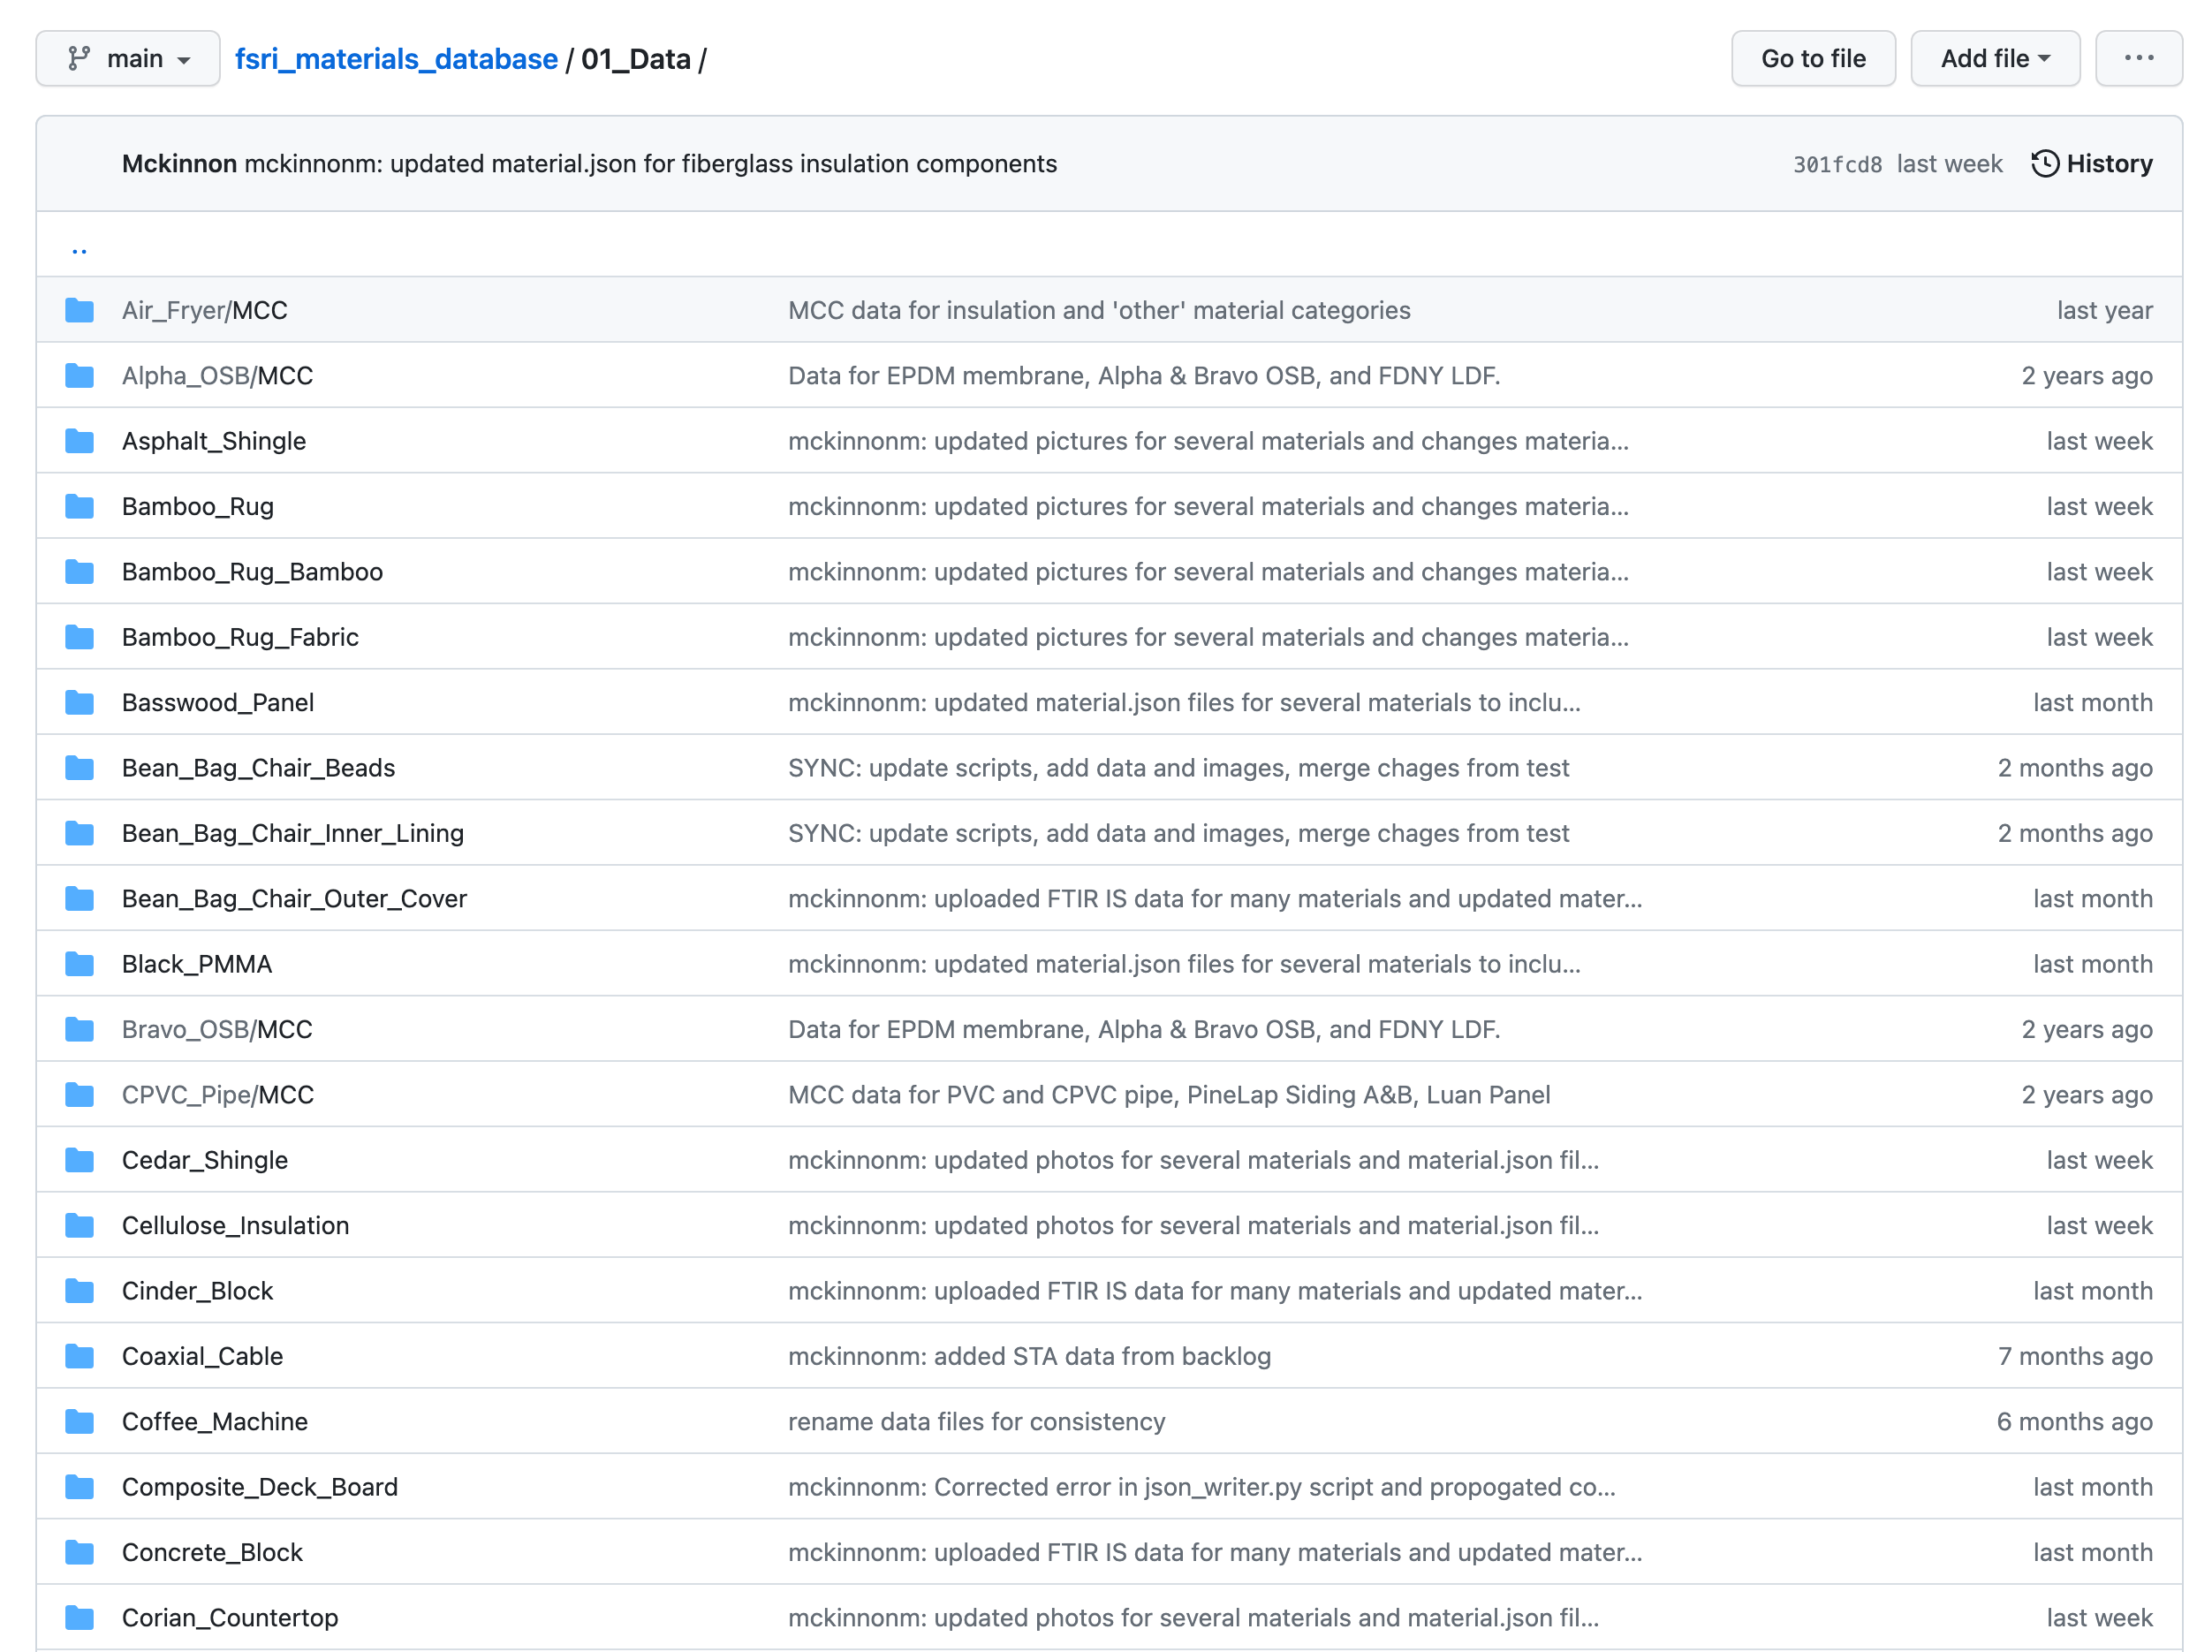
\includegraphics[width=.95\columnwidth]{Figures/partial_materials_github}
\caption[Partial List of Materials from Github Repository]{Partial list of materials from {\bf 01\_Data} in \href{https://github.com/ulfsri/fsri_materials_database}{fsri\_materials\_database} Github repository.}
\label{fig:mat_list}
\end{figure}

The data is organized first by material, next by the short name of test apparatus used, and where applicable additional filtering by test settings. The following sections describe the naming convention used for each of the test apparatus used to generate the data.

\begin{figure}[!ht]
\centering
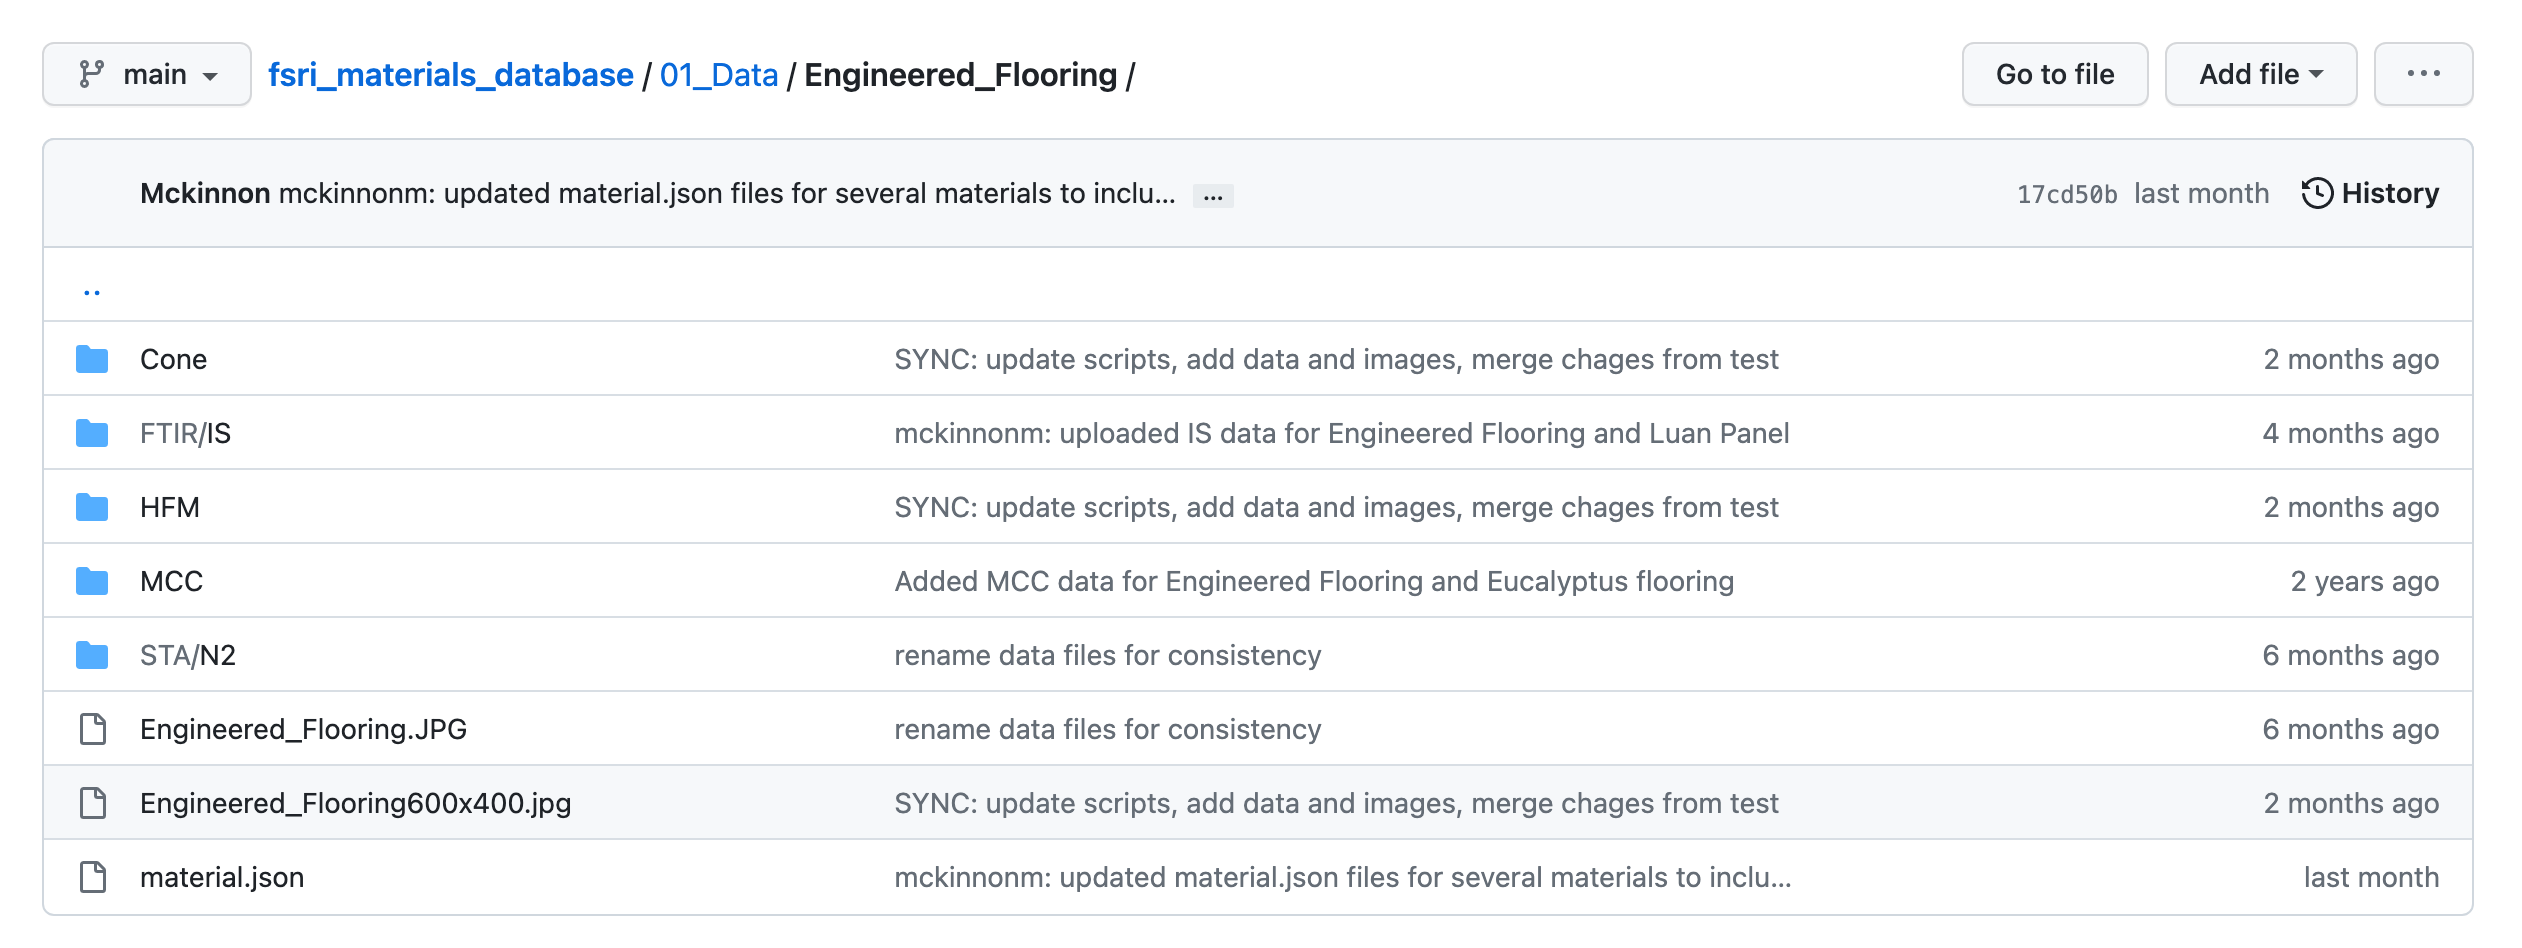
\includegraphics[width=.95\columnwidth]{Figures/engineered_flooring_example}
\caption[Engineered Flooring Material Directory Example]{Example directory structure from engineered flooring.}
\label{fig:mat_list}
\end{figure}

\subsection{Cone Calorimeter (Cone)}
Data file structure includes the material, the short name for the apparatus, heat flux setting and scan/scalar, date of test, and replicate number. Scan is for the raw output data and scalar is for the initial conditions and high-level test parameters.

{\bf Example:} MDF\_Cone\_HF25scalar\_210323\_R1 stands for the first replicate of scalar data generated from a medium density fiber board test in cone calorimeter exposed to 25 kW/m$^2$ on March 23, 2021.
A Cone\_Notes.csv is generated for each material from the plot\_Cone\_data.py script. For materials whose experiments deviated from typical behavior relevant pictures are included in the respective material directory.

\subsection{Fourier Transform Infrared Spectrometer (FTIR)}
The FTIR directory contains subdirectories for the Attenuated Total Reflectance method (ATR) and the Integrating Sphere (IS)
Data file structure for the ATR experiment files includes the material, the abbreviated name for the apparatus, date of test, and replicate number.

{\bf Example:} MDF\_ATR\_210323\_R5 stands for the fifth replicate of data collected with the ATR accessory conducted on June 8, 2021.

Data file structure for the IS experiment files includes the material, the abbreviated name for the apparatus, the measurand, whether the test is a sample measurement or standard reference, date of test, and replicate number.

{\bf Example:} OSB\_IS\_REFLECT\_MEAS\_210623\_R2 stands for the second replicate conducted on oriented strand board to measure spectral reflection in the integrating sphere on June 23, 2021.

\subsection{Heat Flow Meter (HFM)}
Data file structure is the material, the abbreviated name for the apparatus, whether test was dry or wet, whether test was for thermal conductivity or heat capacity, date of test, and replicate number. Scan is for the raw output data and scalar is for the initial conditions and high-level test parameters.

{\bf Example:} OSB\_HFM\_Dry\_Conductivity\_210315\_R3.tst stands for the third replicate of the data generated from an oriented strand board test in the heat flow meter tested dry for thermal conductivity on March 15, 2021.

\subsection{Micro-scale Combustion Calorimeter (MCC)}
Data file structure is the material, the abbreviated name for the apparatus, the heating rate in Kelvin per minute, date of test, and replicate number. Additionally, the final mass of the sample after the test is included in a separate text file named with the appendix 'FINAL\_MASS'.

{\bf Example:} Polyester\_Fabric\_MCC\_30K\_min\_210308\_R1.csv stands for the first replicate of the data generated from a test on polyester fabric in the micro-scale combustion calorimeter tested with a heating rate of 30 Kelvin per minute on March 8, 2021.

\subsection{Simultaneous Thermal Analyzer (STA)}
Data file structure is the material, the abbreviated name for the apparatus, the atmosphere tested in, the heating rate in Kelvin per minute and data/meta, date of test, and replicate number. Data is for the raw output data and meta is for the initial conditions and high-level test parameters.
Example: Polyester\_Batting\_STA\_N2\_3KData\_210215\_R1.csv stands for the first replicate of the data generated from a polyester batting board test in the simultaneous thermal analyzer tested in nitrogen with a heating rate of 3 Kelvin per minute on March 15, 2021.

\subsection{Additional Data Files}

\subsubsection{material.json}
Each material has a json file that links the data stored in the repository and data and graphs produced by the accompanying scripts to the respective landing page for the material on the front-end website. The file also contains a brief description of the material and alternate names of the material to facilitate search.

\subsubsection{Photos}
A full-size and thumbnail photo are included of materials for visualization on front-end website.


\section{Processing Scripts}
\label{sec:scripts}

Python processing scripts exist for analyzing the experimental data to generate derived quantities and to plot the experimental data. The scripts are apparatus specific and cycle through all materials upon execution. Each apparatus has a pair of scripts: data.py and data\_html.py.

The data.py script computes derived quantities, produces reduced data .csv files, and produces .pdf graphs in 03\_Charts/Material/Apparatus.

Derived quantities and/or reduced data files will get dropped into 01\_Data/Material/Apparatus. These files get updated each time the script gets executed.
The data\_html.py script produces interactive .html files that allow interactions such as hover, zoom, and pan and .html tables of relevant processed data. Similar to the data.py script, .html graphs are output to 03\_Charts/Material/Apparatus and can be opened in a web browser.

run\_all.bat and .sh files exist for both the set of data.py scripts and the data\_html.py scripts. These files will execute the respective python scripts for all data in the repository.

If there are issues executing the script, in particular the .sh script, a change mode may be needed. In a command prompt type:
chmod +x run\_all\_data.sh OR chmod +x run\_all\_data\_html.sh
When the scripts, either data.py or data\_html.py, are run, the current version of the repository (i.e., Github hash) is appended to the figure.
To successfully execute the Python scripts in this repository, several additional packages (outside of base Python) will need to be installed. One way to do this is through pip with following commands:

\begin{verbatim}
pip install pandas              #used for data wrangling/processing
pip install numpy               #used for math analysis
pip install scipy               #used for stats analysis
pip install matplotlib          #used for plot styling and pdf plots
pip install plotly              #used for interactive html plots
pip install GitPython           #used for add repo hash to plots
pip install pybaselines         #used for melting analysis in STA
\end{verbatim}

\section{Charts and Tables}
\label{sec:charts}

\chapter{MaP Website}


% \bibliography{../Bibliography/MaP_Database_Bibliography}

\end{document}